\input{"./2ProjectSetup".tex}%
\input{"\DenKrLayoutMainRootDir/2includes/packages/preamble_pre".tex}%
\documentclass[tikz,fontsize=11pt,class=scrbook]{standalone}% I.e. the content from \input{"\DenKrLayoutMainRootDir/2layout/tikz_standalone/preamble_1_class".tex}%
\usepackage{ellipsis}
\input{"\DenKrLayoutBaseRootDir/tikz_standalone/1TikzStandalonePicIncludeThis".tex}%
\DenKrTikzStandalonePre%
%
%
%

\usetikzlibrary{calc}
\usetikzlibrary{decorations.pathreplacing,decorations.markings,shapes.geometric}
\tikzset{naming/.style={align=center,font=\small}}
\tikzset{antenna/.style={insert path={-- coordinate (ant#1) ++(0,0.25) -- +(135:0.25) + (0,0) -- +(45:0.25)}}}
\tikzset{station/.style={naming,draw,shape=dart,shape border rotate=90, minimum width=10mm, minimum height=10mm,outer sep=0pt,inner sep=3pt}}
%\tikzset{mobile/.style={naming,draw,shape=rectangle,minimum width=15mm,minimum height=7.5mm, outer sep=0pt,inner sep=3pt}}
\tikzset{mobile/.style={naming,draw,shape=rectangle,minimum width=12mm,minimum height=6mm, outer sep=0pt,inner sep=3pt}}
\tikzset{radiation/.style={{decorate,decoration={expanding waves,angle=90,segment length=4pt}}}}

\newcommand{\MUE}[1]{%
\begin{tikzpicture}[every node/.append style={rectangle,minimum width=0pt}]
\node [mobile,label={[inner ysep=+.3333em]\dots}] (box) {#1};

%\node [mobile] (box) {#1};
%\node at ($(ant1)!0.5!(ant2)$) {\dots};

\draw ([xshift=.25cm] box.south west) circle (4pt)
      ([xshift=-.25cm]box.south east) circle (4pt);

\fill ([xshift=.25cm] box.south west) circle (1pt)
      ([xshift=-.25cm]box.south east) circle (1pt);

\draw ([xshift=.25cm] box.north west) [antenna=1];
\draw ([xshift=-.25cm]box.north east) [antenna=2];
\end{tikzpicture}
}

\newcommand{\UE}[1]{%
\begin{tikzpicture}[every node/.append style={rectangle,minimum width=0pt}]
\node[mobile] (box) {#1};

\draw ([xshift=.25cm] box.south west) circle (4pt)
      ([xshift=-.25cm]box.south east) circle (4pt);

\fill ([xshift=.25cm] box.south west) circle (1pt)
      ([xshift=-.25cm]box.south east) circle (1pt);

\draw (box.north) [antenna=1];
\end{tikzpicture}
}

\newcommand{\MBS}[1]{%
\begin{tikzpicture}
\node[station] (base) {#1};

%\draw[line join=bevel] (base.110) -- (base.70) -- (base.north west) -- (base.north east) -- cycle;
\draw[line join=bevel] (base.100) -- (base.80) -- (base.110) -- (base.70) -- (base.north west) -- (base.north east);
\draw[line join=bevel] (base.100) -- (base.70) (base.110) -- (base.north east);

% original yshift=.8pt
%\draw[line cap=rect] ([xshift=.5cm,yshift=.3pt] base.north) [antenna=1];
%\draw[line cap=rect] ([yshift=.3pt]ant1 |- base.north) -- node[above,shape=rectangle,inner ysep=+.3333em]{\dots} ([xshift=-.5cm,yshift=.3pt]base.north) [antenna=2];
\draw[line cap=rect] ([xshift=-.1768cm,yshift=.6pt]base.north -| base.right tail) [antenna=1];
\draw[line cap=rect] ([yshift=.6pt]ant1 |- base.north) -- node[above,shape=rectangle,inner ysep=+.3333em]{\dots} ([xshift=.1768cm,yshift=.6pt]base.north -| base.left tail) [antenna=2];

%\draw[line cap=rect] ([yshift=.3pt]ant1 |- base.north) -- ([xshift=-.5cm,yshift=.3pt]base.north) [antenna=2];
%\node at ($(ant1)!0.5!(ant2)$) {\dots};
\end{tikzpicture}
}

\newcommand{\BS}[1]{%
\begin{tikzpicture}
\node[station] (base) {#1};

%\draw[line join=bevel] (base.110) -- (base.70) -- (base.north west) -- (base.north east) -- cycle;
\draw[line join=bevel] (base.100) -- (base.80) -- (base.110) -- (base.70) -- (base.north west) -- (base.north east);
\draw[line join=bevel] (base.100) -- (base.70) (base.110) -- (base.north east);

% original yshift=.8pt
\draw[line cap=rect] ([yshift=0pt]base.north) [antenna=1];
\end{tikzpicture}
}


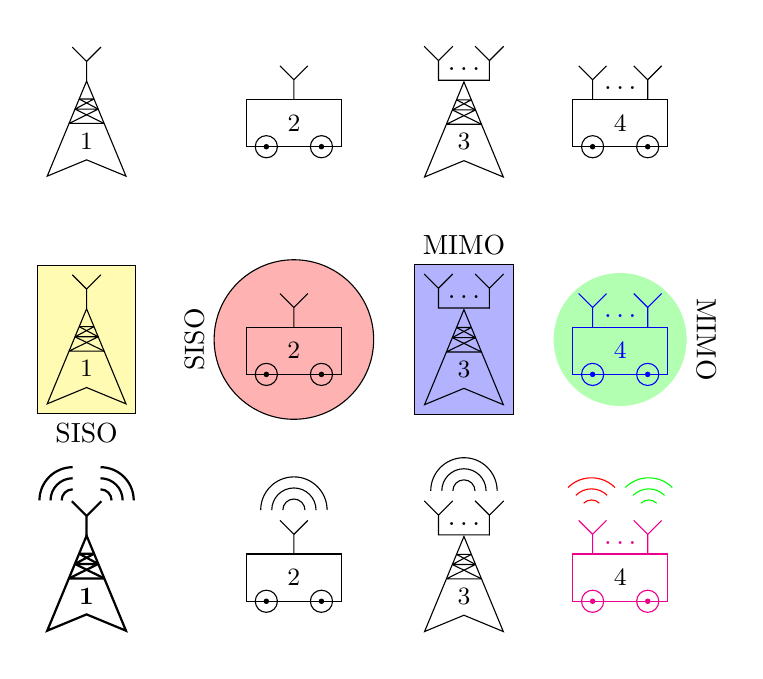
\begin{tikzpicture}[
	scale = 1.0,%Könnte das Makro \tikzpicturescale sein. Siehe in makros.tex
	% (Sollte eigentlich übergeben werden)(Beachte Möglichkeiten der Übergabe;
	% standalone mode=tex vs mode=buildnew)
	auto,
	node distance=\nodedistance
]
%
\matrix[column sep=0.5cm,row sep=0.5cm]
{
    \node{\BS{1}}; & \node{\UE{2}}; & \node{\MBS{3}}; & \node{\MUE{4}};\\
    \node[draw,fill=yellow!30,label=below:SISO] {\BS{1}}; &
    \node[draw,shape=circle,fill=red!30,label={left:\rotatebox{90}{SISO}}] {\UE{2}}; &
    \node[draw,fill=blue!30,label=above:MIMO] {\MBS{3}}; &
    \node[blue,shape=circle,fill=green!30,inner sep=0pt,label={right:\rotatebox{-90}{MIMO}}] {\MUE{4}};\\
    \node[every path/.append style={thick},inner sep=0pt](A){\BS{\textbf{1}}}; & \node(B){\UE{2}}; & \node(C){\MBS{3}}; & \node[magenta,inner sep=0pt](D){\MUE{\textcolor{black}{4}}};\\
};

\draw[thick,radiation,decoration={angle=45}] ([xshift=.1768cm]A.north) -- +(45:0.5);
\draw[thick,radiation,decoration={angle=45}] ([xshift=-.1768cm]A.north) -- +(135:0.5);
\draw[radiation] (B.north) -- +(90:0.5);
\draw[radiation] (C.north) -- +(90:0.5);
\draw[red,radiation,decoration={angle=45}] ([xshift=.25cm,yshift=3pt]D.north west) -- +(90:0.5);
\draw[green,radiation,decoration={angle=45}] ([xshift=-.25cm,yshift=3pt]D.north east) -- +(90:0.5);
%
\end{tikzpicture}%
%
%
\DenKrTikzStandalonePost%